\documentclass[a4paper,14pt]{extarticle}
    \usepackage{amsmath}
    \usepackage{nccmath}
    \usepackage{amsfonts}
    \usepackage{lscape}
    \usepackage[utf8]{inputenc}
    \usepackage{titlepic}
    \usepackage{stackengine}
    \usepackage{lipsum}
    \usepackage{graphicx}
    \usepackage{booktabs}
    \usepackage{cite}
	\usepackage{caption}
	\usepackage{float}
	\usepackage{subcaption}
    \usepackage{multirow}
    \usepackage[top=1in, bottom=1.1in, left=1in, right=1in]{geometry}
    \usepackage{fancyhdr}
    \usepackage{relsize}
    \usepackage{tikz}
    \usetikzlibrary{shapes.geometric,arrows}
	\makeatletter
    \setlength{\@fptop}{0pt}
    \makeatother
    \tikzstyle{startstop} = [rectangle, rounded corners, minimum width = 4cm, minimum height=1cm, text centered,text width = 5cm, draw = black, fill=white!10]    
     \tikzstyle{process} = [rectangle,  minimum width = 4.2cm, minimum height=1.5cm, text centered, text width = 5cm,draw = black, fill = white!10]  
	 \tikzstyle{decision} = [diamond, minimum width = 4cm, minimum height=1cm, text centered,text width = 3cm, draw = black, fill = white!10]  
     \tikzstyle{arrow} = [thick,->,>=stealth]  


\usepackage{titling}
\pretitle{\begin{center}\fontsize{18bp}{18bp}\selectfont}
    \posttitle{\vspace{25bp}\par\includegraphics[width=60mm]{logo.png}\par\end{center}}
\preauthor{\begin{center}\fontsize{14bp}{14bp}\selectfont}
    \postauthor{\par\end{center}}
\predate{\begin{center}}
    \postdate{\par\end{center}}  

\title{\LARGE{\textbf{Development and implementation of material subroutine for fibre reinforced plastics in a commercial FEM software}}\\[0.7cm]\smaller \textbf{Master thesis \\[0.5cm] Winter semester 2018/19}\vspace*{1cm}}


\author{
\vspace{2cm}
\large{Presented by: Arun prakash Ganapathy}
\\[0.4cm]
\large{Supervised by: Dr.-Ing Dominik Laveuve}
\\[0.4cm]
\large{Mat.Nr: 63876}
\\[0.4cm]
\large{E-mail: arun-prakash.ganapathy@student.tu-freiberg.de}}
\date{}
\begin{document}
\maketitle
\section{Introduction}
\subsection{Background and motivation}
\indent\indent Composite materials are made of two or more dissimilar materials of different physical or chemical properties when combined, create a material with properties unlike the individual constituent materials. The earliest use of composite materials date back to 3400 B.C when Mesopotamians glued wood strips at different angles to create plywood. Another notable example is the bow made by Mongols during 1200 A.D, which is made from a combination of bamboo, wood, cattle tendons and silk bonded with natural resin. In the early, 1900s bakelite based composites were developed for its non-conductivity and heat resistant properties and widely used in industrial and consumer applications. Now a days advanced composite materials are widely used in structural design in various industries such as aerospace, automobile, marine, petrochemical etc., due to their superior properties over traditional engineering materials.\\
\begin{figure}[htbp]
\begin{center}
\includegraphics[width=0.8\textwidth]{{composite plane.jpg}}
 \caption{Composite materials used in a Boeing 787 'Dreamliner'}
 \label{fig:Composite plane}
\end{center}
\end{figure}\\
 Composite material are attractive because of their high strength, stiffness, high stiffness-to-density ratio, light weight properties etc., Another important reason for using composite materials is the ability to tailor the stiffness and strength to specific design load flexibly. Despite their superior physical properties, composite materials are fragile and can be easily damaged from number of sources, both during initial processing and in operation. Since composite materials possess elastic brittle properties with negligible margin of safety through ductility as offered by metals and accumulate damage before structural collapse, the development of damage must be understood for predicting failure of such materials. For example fibre-reinforced plastics exhibit local damage such as fibre breakage, matrix cracks, fibre matrix debonds etc., under normal operating conditions which may contribute to the failure. Therefore the ability to predict the initiation and growth of damage is important for predicting the performance of the composite materials for safe and reliable use of such materials. Continuum damage mechanics (CDM) has been considered as a reliable candidate for creating numerical models which predict the onset and evolution of the damage in the composite materials.
\newpage
\section{Continuum damage mechanics}
\indent\indent\indent Continuum damage mechanics (CDM) is a theory for analyzing damage and fracture processes in materials from continuum mechanics point of view. Continuum damage mechanics (CDM) provides a continuum perspective for microflaws initiation, propagation, and their coalescence that eventually results in macroscopic faults and fractures. CDM uses state variables to represent the effect of damage on the stiffness and remaining life of the material that is damaging as a result of load and ageing. A Damage activation function is required to predict the initiation of damage. Damage evolution does not progress spontaneously after initiation therefore a mathematical model is required.  

\subsection{Damage}
\indent\indent\indent  Consider a body B of Fig. \ref{fig:Damage}  where a crack of length a has developed due to an external load F.  If we take an arbitrary point P($x$) near the crack tip, a number of microscopic cavities or microcracks would be observed around the region.
These cavities can be nucleated usually as a result of breakage of atomic bonds, or of some defects in atomic array. From microscopic point of view, fracture of materials is a process of nucleation of microcavities or microcracks due to the breakage of atomic bonds. From macroscopic point of view, it is a process of extension of cracks brought about by the coalescence of these microcracks.
\begin{figure}[htbp]
\begin{center}
\includegraphics[width=0.4\textwidth]{{1. Damage.png}}
 \caption{Scales of damage observation}
 \label{fig:Damage}
\end{center}
\end{figure}
 From mesoscopic point of view, which exists between microscopic and macroscopic scale, it is a process of nucleation, growth and the coalescence of microscopic cavities leads to the initiation of macroscopic crack. The development of microscopic, mesoscopic and the macroscopic processes of fracture in materials together with the resulting deterioration in their mechanical properties is called damage. Continuum damage mechanics, in particular, aims at the analysis of the damage development in mesoscopic and macroscopic fracture processes in the framework of continuum mechanics.

The seperation of atomic bonds is induced either by shear or tensile decohesion. However the separation of material at the microscopic level consists of four damage mechanisms namely Cleavage, Growth and Coalescence of Microvoids, Glide plane decohesion and Void Growth due to Grain-Boundary diffusion.  The aspects of damage vary largely by difference in materials and loading conditions. The damage may be classified phenomenologically as follows
\begin{itemize}
\item Ductile Damage
\item Brittle Damage
\item Creep Damage
\item Low Cycle Fatigue
\item Very Low Cycle Fatigue
\item High Cycle fatigue damage
\item Very High Cycle fatigue damage
\item Creep Damage
\end{itemize}
\subsection{Representative Volume Element(RVE)}
\indent\indent\indent  In order to discuss the effects of microscopic discontinuities in  a material by means of CDM we must homogenize the mechanical effects of microstructure and represent them as a macroscopic continuous field in the material. For this purpose we take a small region of a mesoscale around the material point P($x$) in a body B as showin in Fig. \ref{fig:Damage}. We assume that the  material with discontinuous structures in this region can be statistically homogeneous and the mechanical state of the material in this region can be represented by the statistical average of the mechanical variables in that region. This region is said to be the Representative Volume Element(RVE). For such RVE, the following two conditions must be satisfied:
\begin{itemize}
\item  For the material in the RVE to be statistically homogeneous, the RVE should be large enough to contain a sufficient number of discontinuities
\item In order to represent a non-uniform macroscopic mechanical field by means of a continuum, the size of RVE should be sufficiently small so that the variation of the macroscopic variable in it may be insignificantly small
\end{itemize}
The size of RVE depends on the microstructure of the relevant material and their typical sizes are as follows
\begin{itemize}
\item Metals and ceramics  \;    -    \; 0.1$mm^3$
\item Polymer and composites \;   -   \; 1$mm^3$
\item Timber\; - \; 10$mm^3$
\item Concrete \; - \; 100$mm^3$
\end{itemize}

\subsection{Concept of Continuum damage mechanics (CDM)}
\indent\indent\indent The basic concept of CDM is that the  microstructural defects in a material can be represented by a set of damage variables.  Continuum damage mechanics first represent the damage state of a material in terms of properly defined damage variables and then describe the mechanical behaviour of the damaged material and then development of damage by use of these damage variables. The mechanical behaviour of a damaged material can be described using the notion of effective stress, together with hypothesis of mechanical equivalence between damaged and undamaged material. The concept of effective stress and mechanical equivalence will be discussed in the following sections.
\subsubsection{Modelling by Effective Area Reduction}
Let us consider a body B of Fig. (\ref{fig:Damage2}) and take a representative volume element(RVE) at an arbitrary point $P(x)$ in B. If the total void area in $dA$ is  $ dA_{D} $, the mechanical effect of $dA$ will be decreased by $dA_{D}$. Then the area,
\begin{equation}
  d\tilde{A} = dA  - dA_{D}
  \label{eqn:da} 
\end{equation}
may be interpreted as the area which carries the internal force and is called as $effective$ $area$. Thus the damage variable D can be specified as 
\begin{equation}
 \label{eqn:D}
  D = \frac{dA - d\tilde{A}}{dA} = \frac{dA_{D}}{dA}
\end{equation}
where the damage variable D takes value between 0 and 1 ($0 \leq D \leq 1$). $D = 0$ representing initial undamaged state and $D=1$ represents fully damaged state.
\begin{figure}[htbp]
\begin{center}
\includegraphics[width=0.8\textwidth]{{Damage2.png}}
 \caption{Effective area reduction due to microcracks}
 \label{fig:Damage2}
 \end{center}
\end{figure}
Suppose a cylindrical bar of cross-sectional area $dA$ is subject to a tensile load $dF$ the actual load carrying area is $ d\tilde{A}$ rather than $dA$. According to eqn (\ref{eqn:da}) and (\ref{eqn:D}) the effective area $ d\tilde{A}$ is given by,
\begin{equation}
\label{eqn:da_t}
 d\tilde{A} = (1-D)dA
\end{equation}
The decrease in load-carrying area increase the effect of stress $\sigma$ induced by the external force $dF$. Due to eqn \ref{eqn:da_t} the magnified stress $\tilde{\sigma}$ is given by,
\begin{equation}
\label{eqn:sig_t}
\tilde{\sigma} = \frac{dF}{d\tilde{A}} = \frac{\sigma}{1 - D}
\end{equation} 

Since the stress $\tilde{\sigma}$ represents the effect of stress magnified by the net area reduction due to damage, it is called as $effective$ $stress$. From eqn (\ref{eqn:da_t}) and (\ref{eqn:sig_t}) we can postulate that the damaged cylindrical bar of Fig.(\ref{fig:Damage3}b) with the cross-sectional area $dA$ subject to force $dF$ is mechanically equivalent to the fictious undamaged bar of Fig.(\ref{fig:Damage3}c) which is subject to force $dF$ , has the cross-sectional area $ {d\tilde{A}} $ and hence stress has the stress $\tilde{\sigma}$  
\begin{figure}[htbp]
\begin{center}
\includegraphics[width=0.8\textwidth]{{3. Damage_cylinder.png}}
 \caption{Damage of bar under tensile load}
 \label{fig:Damage3}
 \end{center}
\end{figure}

\subsubsection{Modelling by variation of elastic modulus} 
\indent\indent\indent Since the development of microcracks induces the reduction in stiffness of material, the damage state can be characterized by variation in elastic modulus. Let us consider the bar (b) and (c) of Fig. (\ref{fig:Damage3}) are in damaged and fictitious undamaged state respectively. Then the elastic strain $\epsilon$ in the bar (c) caused by stress $\tilde{\sigma}$ should be equal to the $\epsilon$ of the bar (b) under stress $\sigma$; i.e.,\\
\begin{equation}
\label{eqn:sig_t2}
   \tilde{\sigma} = E_{0}\epsilon, \;\;  \sigma = E(D)\epsilon 
\end{equation}
\\
\begin{equation}
\label{eqn:epsilon}
\epsilon = \frac{\sigma}{E(D)} = \frac{\tilde{\sigma}}{E_{0}}
\end{equation}
where $E_{0}$ and $E(D)$ denote young's modulus of the material in the initial undamaged state and that in damaged state after loading, respectively. Therefore, eqn. (\ref{eqn:epsilon}) defines another effective stress\\
\begin{equation}
\label{eqn:epsilon2}
\epsilon = \frac{E_{0}}{E(D)}\sigma
\end{equation}
By combining Eqn. (\ref{eqn:sig_t}) and (\ref{eqn:epsilon}) we get,
\begin{equation}
\label{eqn:E(d)}
E(D) = (1 - D) E_{0}
\end{equation}
\begin{equation}
\label{eqn:D2}
D  = 1 - \frac{E(D)}{E_{0}}
\end{equation}
Therefore, the damage variable $D$ is characterized by the variation in Young's modulus $E(D)$. The modelling of damage by means of reduction in stiffness can be applied also the anisotropic damage of brittle materials like composite materials, concrete, rocks etc.,
\subsection{Mechanical representation of three dimensional damage state}
\indent\indent\indent The deformation of a material basically depends on the direction of applied stress or strain and hence it is an anisotropic phenomenon. Therefore different theories have been developed for modelling 3-D anisotropic damage phenomenon. Some fundamental theories that describes 3-D damage state are given below 
\subsubsection{Scalar Damage Variable}
\indent\indent\indent In case of random or isotropic distribution of microcracks or voids , the damage state is usually considered as isotropic. the damage state in this case may be represented by means of scalar damage variable D. When microvoids  have oriented distribution the damage state is anisotropic and the scalar damage variable cannot be applied accurately. However, when void density is small the global mechanical properties can be approximated as nearly isotropic. Thus isotropic damage theory based on isotropic damage variable has been often applied to 3-D problems of creep, elastic-plastic, ductile and fatigue damage
\subsubsection{Plural Scalar damage variables}
\indent\indent\indent A single scalar damage variable is often insufficient to describe the variation in mechanical properties of the damaged materials, even if the distribution of microcracks are isotropic. Plural scalar damage variables are often employed to characterize several different microscopic mechanisms of the relevant damage development.
\subsubsection{Vector damage variable}
\indent\indent\indent The damage state can be specified by the decrease in load carrying effective area due to void development. Hence it is easy to postulate a vector damage variable. Kachanov (1974, 1986) tried to extend the definition of damage to anisotropic damage by noting a surface element in an arbitrary direction $n$, he proposed a vector damage variable $ \omega = \omega_{n}n$, where $\omega_{n}$ is the effective area fraction. 
\subsubsection{Damage tensor of second order}
\indent\indent\indent In order to describe an anisotropic damage state, damage variable of second or higher order tensor is required. Eqn.(\ref{eqn:da_t}) suggests that the damage state (1 - D) is specified by the transformation of the surface element $dA$ of Fig. (\ref{fig:Damage3}b) of the damage state into the corresponding surface element $d\tilde{A}$ in the fictitious undamaged state of Fig.(\ref{fig:Damage3}c). 
\begin{figure}[htbp]
\begin{center}
\includegraphics[width=0.5\textwidth]{{4. Damage.png}}
 \caption{Surface element in RVE of a damaged material}
 \label{fig:Damage4}
 \end{center}
\end{figure}
In order to express damage as a second order tensor, we first consider an arbitrary surface element $PQR$ in RVE in the current damaged configuration $B_{t}$ of Fig.(\ref{fig:Damage4}a) . The unit normal vector and area of $PQR$ are denoted by $\nu$ and $dA$. We further postulate the fictitious undamaged configuration $B_{f}$ of Fig.(\ref{fig:Damage4}b) mechanically equivalent to $B_{t}$, and the surface element and its area vector are denoted by $\tilde{P}\tilde{Q}\tilde{R}$ and $\tilde{\nu}d\tilde{A}$ respectively. According to Eqn.(\ref{eqn:da_t}) the damage variable of second-order tensor $D$ should be defined by linear transformation from area vector $\nu dA$ in $B_{t}$ into $\tilde{\nu}d\tilde{A}$ in $B_{f}$, i.e.,
\begin{equation}
\label{eqn:second_order_tensor}
\tilde{\nu}d\tilde{A} = (I - D)\nu dA
\end{equation}
where $I$ is the second order identity tensor. Since the damage tensor $D$ is symmetric, it can be expressed by its spectral decomposition
\begin{equation}
\label{eqn:damage_2nd_order}
D = \sum_{i = 1}^{3} D_{i}n_{i}  \otimes D_{i}n_{i}
\end{equation}
where $D_{i}$ and $n_{i}$ are the principal value and principal direction of $D$. 
\subsubsection{Damage tensors of Fourth order and eighth order}
\indent\indent\indent Let us consider the fourth-order elastic modulus tensor of an undamaged and the damaged material be denoted by $\mathbb{C}_{0}$ and $\mathbb{C}(D)$. Then the elastic constitutive equation of these materials is given by \\
\begin{equation}
\label{eqn:4thorder_sigma}
  \sigma  =  \mathbb{C}_{0} : \epsilon  \;\;\;  \sigma = \mathbb{C}(D) : \epsilon
\end{equation}
where (:) denotes the double contraction. Since the the elastic strain in a damaged material under stress $\sigma$ is equal to the equivalent fictitious undamaged material subject to effective stress $\sigma$, we have
\begin{equation}
\label{eqn:4thorder_tilde_sigma}
 \tilde{\sigma}  = \mathbb{C}_{0} : \epsilon
\end{equation}
Form Eqn.(\ref{eqn:4thorder_sigma}) and (\ref{eqn:4thorder_tilde_sigma}) we can represent effective stress as 
\begin{equation}
\tilde{\sigma}  = [\mathbb{C}_{0} : \mathbb{C}(D)^{-1}] : \sigma
\end{equation}
From equation (\ref{eqn:4thorder_sigma}), the damage tensor $D$ may be viewed as an eighth-order tensor which transforms fourth order elasticity tensor $\mathbb{C}_{0}$ of an undamaged material into another fourth-order tensor $\mathbb{C}(D)$ of the damaged material. Since mathematical operation of eighth-order tensor is highly complicated an alternative fourth-order damage tensor $\mathbb{D}$ has been proposed and the transformation between elastic moduli is given by,
\begin{equation}
\mathbb{C}(\mathbb{D})  =  (\mathbb{I}  - \mathbb{D}) : \mathbb{C}_{0}
\end{equation}
where $\mathbb{I}$ denotes the fourth-order identity tensor. The fourth order damage tesnor $\mathbb{D}$ and the effecctive stress tensor $\tilde{\sigma}$ are given by the following relations
\begin{equation}
\mathbb{D}  = \mathbb{I} - \mathbb{C}(\mathbb{D}) : \mathbb{C}_{0}^{-1}
\end{equation}\\
\begin{equation}
\label{eqn:4thorder_effective_stress}
\tilde{\sigma} =  (\mathbb{I} - \mathbb{D})^{-1} : \sigma
\end{equation}
Since the damage tensor $\mathbb{D}$ given by Eqn(\ref{eqn:4thorder_effective_stress}) is asymmetric, Chaboche(1993) later employed an alternative transformation,
\begin{equation}
\mathbb{C}(\hat{\mathbb{D}}) = \frac{1}{2}\; [(\mathbb{I} - \hat{\mathbb{D}}) : \mathbb{C}_{0} + \mathbb{C}_{0} : (\mathbb{I} - \hat{\mathbb{D}}  ]
\end{equation}
and proposed a new fourth-order symmetric tensor $\hat{\mathbb{D}}$.
\subsection{Effective Stress Tensors}
\indent\indent\indent The effective stresses are  used to describe the mechanical behaviour of the damaged material. Some of the effective stresses postulated in damage mechanics are given below
\subsubsection{Effective Stress Tensor for Isotropic Damage}
\indent\indent\indent If the damage state is isotropic then the effective stress tensor of three-dimensional state is given by
\begin{equation}
\tilde{\sigma} = (1 - D)^{-1} \; \sigma
\end{equation}
where D is the scalar damage variable and $\sigma$ is the Cauchy stress tensor. This effective stress simplifies damage theory and can be applied to number of damage problems like ductile damage. But this cannot be applied to damage of significant anisotropy, such as brittle damage due to microcrack distribution\\
\subsubsection{Asymmetric Effective Stress Tensor for Anisotropic Damage}
\indent\indent\indent The increase in stress effect caused by the net area reduction in case of anisotropic damage is given by
\begin{equation}
\tilde{\sigma} = (I - D)^{-1} \; \sigma
\end{equation}
where I and D are second order identity tensor and the second order damage tensor respectively. In the actual development of anisotropic damage, the stress induced in RVE of damage material is asymmetric. But asymmetric stress tensor makes the numerical analysis complicated and thus different methods of symmetrization has been proposed. Few of them are described as follows

\subsubsection{Symmetrized Effective Stress Tensor for Anisotropic Damage 1 (Murakami and Ohno 1981)} 
\indent\indent\indent A simple symmetrization procedure of Eq.(\ref{eqn: Murakami and Ohno}), the symmetric part of the Cartesian decomposition of Eq.(\ref{eqn: Murakami and Ohno}) gives,
\begin{equation}
\label{eqn: Murakami and Ohno}
\tilde{\sigma} = \frac{1}{2} [(I - D)^{-1}\;\sigma + \sigma(I - D)^{-1}]
\end{equation}\\
\subsubsection{Symmetrized Effective Stress Tensor for Anisotropic Damage 2 (Cordebois and Sidoroff 1982a, b)}
\indent\indent\indent Another form of symmetrization was proposed by Cordebois and Sidoroff:
\begin{equation}
\label{eqn:Cordebois and Sidoroff }
\tilde{\sigma} =  (I - D)^{-1/2}\sigma(I - D)^{-1/2}
\end{equation}
where $\sigma$ and $D$ are co-axial. Moreover, unless the development of damage is large, the difference between these effective stresses are known to be insignificant.\\
\subsubsection{Symmetrized Effective Stress Tensor for Anisotropic Damage 3 ((Betten 1986)}
\indent\indent\indent  Betten derived another effective stress tensor , ie.,
\begin{equation}
\label{eqn:Betten }
\tilde{\sigma} =  (I - D)^{-1}\sigma(I - D)^{-1}
\end{equation} 
Since tensors $(I - D)^{-1}$ and $(I - D)^{-1/2}$ are both second-order symmetric positive tensor, there is no essential difference between Eqs.(\ref{eqn:Cordebois and Sidoroff }) and (\ref{eqn:Betten }).

\subsection{Matrix Representation of Damage effect tensors}\label{Matrix Representation of Damage effect tensors}
\indent\indent\indent The general form of an effective stress tensor $\tilde{\sigma}$ is given by the damage effect tensor $\mathbb{M}$ and the corresponding Cauchy stress tensor $\sigma$, i.e.,
\begin{equation}
\tilde{\sigma}  = \mathbb{M} \; :  \sigma 
\label{eqn:effective_stress_tensor} 
\end{equation}
It is convenient to express the tensors in the form of matrices and then execute the tensor operations as a matrix calculus.. To simplify this procedure, we take an orthonormal basis ${n_{i}}$ with principal directions $n_{i}$ of the second-order symmetric damage tensor $D$, and represent the the tensor in terms of their component to this basis. According to voigt notation, the second-order symmetric tensor $\sigma$ and the related effective stress $\tilde{\sigma}$ are expressed by column vector of six dimension:
\begin{equation}
   [\sigma_{P}]  \equiv  [\sigma_{11} \;\; \sigma_{22} \;\;\sigma_{33} \;\;\sigma_{12} \;\;\sigma_{13} \;\;\sigma_{23} ]^{T}
\end{equation}

\begin{equation}
   [\tilde{\sigma_{P}}]  \equiv  [\tilde{\sigma_{11}} \;\; \tilde{\sigma_{22}} \;\;\tilde{\sigma_{33}} \;\;\tilde{\sigma_{12}} \;\;\tilde{\sigma_{13}} \;\;\tilde{\sigma_{23}} ]^{T}
\end{equation}
\\
The damage effect tensor $\mathbb{M}$ can be represented as symmetric matrix. By representing first two indices $ij$ and the succeeding two indices $kl$ of the tensor by $p$ and $q$ ($p,q$ = 1,2,...,6), respectively, the components of $\mathbb{M}$
are expressed by a six by six matrix 
\\
\\
$$
[\mathbb{M}_{pq}] \equiv   
 \begin{bmatrix}
  M_{1111}\; & M_{1122}\; & M_{1133}\; & M_{1123}\; & M_{1131}\; & M_{1112} \\
  \\
  M_{2211}\; & M_{2222}\; & M_{2233}\; & M_{2223}\; & M_{2231}\; & M_{2212} \\
   \\
  M_{3311}\; & M_{3322}\; & M_{3333}\; & M_{3323}\; & M_{3331}\; & M_{3312} \\
   \\
  M_{2311}\; & M_{2322}\; & M_{2333}\; & M_{2323}\; & M_{2331}\; & M_{2312} \\
   \\
  M_{3111}\; & M_{3122}\; & M_{3133}\; & M_{3123}\; & M_{3131}\; & M_{3112} \\
   \\
  M_{1211}\; & M_{1222}\; & M_{1233}\; & M_{1223}\; & M_{1231}\; & M_{1212} 
   \\ 
 \end{bmatrix}
  $$
 \\

By means of the matrix representation, we have the matrix form
\begin{equation}
[\tilde{\sigma_{P}}] \equiv [\mathbb{M}_{pq}]\;: [\sigma_{P}]
\label{eqn:Matrix_rep_damage_effect_tensor}
\end{equation}
\\
Matrix representation of the damage effect tensor of Eq.(\ref{eqn:Matrix_rep_damage_effect_tensor}) is shown below
\\
$$
[\mathbb{M}_{pq}] \equiv   
 \begin{bmatrix}
  \Phi_{1} \; & 0 \; & 0 \; & 0 \; & 0\; & 0 \\
  \\
  0\; & \Phi_{2}\; & 0\; & 0\; & 0\; & 0 \\
  \\
  0\; & 0 \; & \Phi_{3}\; & 0\; & 0\; & 0 \\
  \\
  0\; & 0\; & 0\; & \frac{\Phi_{2} + \Phi_{3} }{2}\; & 0\; & 0 \\
  \\
  0\; & 0\; & 0\; & 0\; & \frac{\Phi_{1} + \Phi_{3} }{2}\; & 0 \\
  \\
  0\; & 0\; & 0\; & 0\; & 0\; & \frac{\Phi_{1} + \Phi_{2} }{2}  
  \\
 \end{bmatrix}
 \label{Damage_effect_tensor}
 $$
\\
\begin{equation}
\Phi_{i}  =  (1 - D_{i})^{-1}, \;\; (i = 1,2,3)
\end{equation}
or
\begin{equation}
M_{11}^{(1)}  =  \frac{1}{1 - D_{1}},....,M_{66}^{(1)}  = \frac{1}{2}( \frac{1}{1 - D_{1}} + \frac{1}{1 - D_{2}}) 
\end{equation}

\subsection{Hypothesis of Strain Equivalence}\label{Hypothesis of Strain Equivalence}

\indent\indent\indent The inelastic constitutive equation of a damaged material is given by the corresponding constitutive equation for an undamaged material by replacing the stress tensor $\sigma$ in the equation with the corresponding effective stress tensor $\tilde{\sigma}$. In Fig. the effect of stress $\sigma$ acting on RVE in the current damaged configuration $B_{t}$ is equivalent to that of the stress $\tilde{\sigma}$ in the fictitious undamaged configuration. Therefore the deformation of the damaged material subject to stress $\sigma$ should be equal to that of the fictitious undamaged material subject to stress $\tilde{\sigma}$. Suppose the constitutive equation of an undamaged inelastic material is given by
\begin{equation}
  \epsilon = F_{0}(\sigma, \alpha)
\end{equation} 
or
\begin{equation}
  \dot{\epsilon} = F_{0}(\sigma, \alpha)
\end{equation}

where $\alpha$ is an internal variable representing the internal change other than damage. and ($\dot{}$) denotes the material time derivative
\begin{figure}[htbp]
\begin{center}
\includegraphics[width=0.8\textwidth]{{6. Strain_eq.png}}
 \caption{Hypothesis of strain equivalence}
 \label{fig:Strain_eq}
 \end{center}
\end{figure}
Then according to hypothesis of strain equivalence, the inelastic constitutive equation of the damaged material represented by a damage variable $D$ should be given by replacing $\sigma$ of Eq.(25) with the effective stress $\tilde{\sigma}$ i.e.,

\begin{equation}
    	\epsilon = F(\sigma, D, \alpha)  = F_{0}(\tilde{\sigma}, \alpha)
\end{equation}

or 
\begin{equation}
    	\dot{\epsilon} = F(\sigma, D, \alpha)  = F_{0}(\tilde{\sigma}, \alpha)
\end{equation}

In case of elastic deformation, constitutive equations for an undamaged and damaged material is given by
\begin{equation}
\epsilon = \mathbb{S}_{0}\; : \sigma,
\end{equation}\\
\begin{equation}
\epsilon = \mathbb{S}(D)\; : \sigma,
\end{equation}
where $\mathbb{S}_{0}$ and $\mathbb{S}(D)$  are fourth-order elastic compliance tensors of the materials. Therefore, according to the hypothesis of strain equivalence the elastic constitutive equation of the damaged material and the compliance tensor is given by 
\begin{equation}
\epsilon = \mathbb{S}_{0}\; : \tilde{\sigma}  =  [\mathbb{S}_{0}\;: \mathbb{M} (D)]\;: \sigma = \mathbb{S}(D)\; : \sigma
\end{equation}
\begin{equation}
\mathbb{S}(D) = \mathbb{S}_{0}\; : \mathbb{M} (D)
 \label{eqn:S_HSeq}
\end{equation}
where $\mathbb{M} (D)$ is the damage effect tensor which is given by 
\begin{equation}
\mathbb{M} (D)  = \mathbb{S}_{0}^{-1} \; : \mathbb{S}(D) 
\end{equation}
The resulting compliance tensor of Eq.(\ref{eqn:S_HSeq}) has inconvenience of its asymmetry which can resolved by taking another variable $D^{*}$ besides $D$.
\begin{equation}
	\mathbb{S}^{*} (D)  = \frac{1}{2} [ \mathbb{S}_{0} \; :  \mathbb{M} (D^{*}) + \mathbb{M}^{T} (D^{*})\; : \mathbb{S}_{0} ]
\end{equation}
and
\begin{equation}
	\mathbb{M} (D^{*})  =  \frac{1}{2}  [ \mathbb{M} (D^{*}) +  \mathbb{S}_{0}^{-1}\; : \mathbb{M}^{T} (D^{*})\; : \mathbb{S}_{0} ]
\end{equation}
\subsection{Hypothesis of strain energy equivalence}\label{Hypothesis of strain energy equivalence}
\indent\indent\indent Let us consider an elastic-plastic material, and represent the internal change due to plastic deformation by an internal state variable $\alpha$. The complementary strain energy functions of the material at undamaged and damaged state are given, respectively as follows
\\
\begin{equation}
V_{0}(\sigma,\alpha) = \frac{1}{2}\sigma : \mathbb{S}_{0} : \sigma \; - \; \phi(\alpha)
\end{equation}
\\
\begin{equation}
V(\sigma,D,\alpha) = \frac{1}{2}\sigma : \mathbb{S}(D) : \sigma \; - \; \phi(\alpha)
\end{equation}
\\
Thus the constitutive equation for the undamaged and damaged material 
\\
\begin{equation}
\epsilon = \frac{\partial V_{0} }{\partial \sigma} = \mathbb{S}_{0} : \sigma
\end{equation}
\\
\begin{equation}
\epsilon = \frac{\partial V }{\partial \sigma} = \mathbb{S}(D) : \sigma
\label{eqn:Strain_energy_eq}
\end{equation}

\begin{figure}[htbp]
\begin{center}
\includegraphics[width=0.8\textwidth]{{7.Strain_energy_eq.png}}
 \caption{Hypothesis of strain energy equivalence}
 \label{fig:Strain_energy_eq}
 \end{center}
\end{figure}

Suppose a damaged material of Fig.(\ref{fig:Strain_energy_eq})a subject to stress $\sigma$, and represent the damage and internal state due to inelastic deformation by $D$ and $\alpha$, respectively. Then the strain energy function $V(\sigma,D,\alpha)$ of the damaged material is given by replacing $\sigma$ in the corresponding function $V_{0}(\sigma,\alpha)$ of the undamaged material of Fig.(\ref{fig:Strain_energy_eq})b with effective stress $\tilde{\sigma}$
\\
\begin{equation*}
V(\sigma,D,\alpha) \; = \; V_{0}(\tilde{\sigma},\alpha)
\end{equation*}
\\
By the use of this hypothesis, the elastic strain of Eq.(\ref{eqn:Strain_energy_eq}) leads to
\\
\begin{equation*}
\epsilon \; = \; \frac{\partial V(\sigma,D,\alpha)}{\partial \sigma} = \mathbb{S}(D) : \sigma 
\end{equation*}
\\
\begin{equation*}
\;\;\;\;\;\;\;\;\;\; = \; \frac{\partial V_{0}(\tilde{\sigma},\alpha)}{\partial \sigma} = \frac{\partial}{\partial \sigma}(\frac{1}{2}\tilde{\sigma} : \mathbb{S}_{0} : \tilde{\sigma} )
\end{equation*}
\\
\begin{equation*}
\;\;\;\;\;\;\;\;\;\;\;\;\;\;\;\;\;\; = \; \frac{1}{2}\frac{\partial}{\partial \sigma} [(\mathbb{M}(D):\sigma) : \mathbb{S}_{0} : (\mathbb{M}(D):\sigma)]
\end{equation*}
\\
\begin{equation}
= \;[\mathbb{M}^{T}(D) : \mathbb{S}_{0} : \mathbb{M}(D)]
\label{M_eqn}
\end{equation}
\\
From Eq.(\ref{M_eqn}), the elastic compliance tensor of the damaged material is given as follows
\\
\begin{equation}
\mathbb{S}(D) \; = \; \mathbb{M}^{T}(D) : \mathbb{S}_{0} : \mathbb{M}(D)
\label{eqn: S_HSEeq}
\end{equation}
In relation to the effective stress tensor $\tilde{\sigma}$ of Eqn.(\ref{eqn:effective_stress_tensor}) we may define a new effective strain tensor
\\
\begin{equation}
\tilde{\epsilon} \; = \; \mathbb{M}^{-T}(D) : \epsilon
\end{equation}
\\
Then the complementary strain energy function and the elastic constitutive equation can be written also in the form
\\
\begin{equation}
V = \frac{1}{2}\sigma : \epsilon \; - \; \phi(\alpha) = \frac{1}{2}\tilde{\sigma} : \tilde{\epsilon} \; - \; \phi(\alpha)
\end{equation}
\\
\begin{equation}
\tilde{\epsilon} \; = \; \mathbb{S}_{0} : \tilde{\sigma}
\end{equation}
\newpage 
\subsection{Elastic Constitutive equation and Elastic modulus tensor}
\subsubsection{Isotropic materials}
\indent\indent\indent Isotropic materials are the materials which exhibit same material properties in all directions at a given point. This means when a load is applied at any point in the material it will exhibit same stress, strain, strength, hardness etc., The elastic constitutive equation of the isotropic material has the form, 
\begin{equation}
  \sigma = \mathbb{C}_{0} : \epsilon   \;\;\;  \sigma_{ij}  =  C^{0}_{ijkl}\epsilon_{kl},
\end{equation}
\begin{equation}
\mathbb{C}_{0} =  \lambda I \otimes I  +  2\mu ´\mathbb{I}^{s}
\end{equation}\\
\\
or
\begin{equation}
C^{0}_{ijkl} = \lambda\delta_{ij}\delta_{kl}  +  \mu(\delta_{ik}\delta_{jl}+\delta_{il}\delta_{jk})
\end{equation}

The fourth-order elastic modulus tensor $\mathbb{C}_{0}$ can be represented in matrix form as 
\\
\\
$$
[C^{0}_{pq}] =  \frac{E}{(1 + \nu)(1 - 2\nu)}
 \begin{bmatrix}
  1 - \nu \; & \nu \;& \nu\; & 0 \;& 0 \;& 0 \\
  \\
  \nu \; & 1-\nu \;& \nu \;& 0 \;& 0 \;& 0 \\
  \\
  \nu \;& \nu \;& 1-\nu \;& 0 \;& 0 \;& 0 \\
  \\
  0 \;& \nu \;& \nu \;& 1 - 2\nu \;& 0 \;& 0 \\
  \\
  0 \;& \nu \;& \nu \;& 0 \;& 1 - 2\nu\;& 0 \\
  \\
  0\;& \nu \;& \nu \;& 0 \;& 0 \;&1 - 2\nu  
 \end{bmatrix}
 $$
 \\
 \\
\subsubsection{Orthotropic materials}
\indent\indent\indent Orthotropic materials are materials which exhibit different material properties along three mutually-orthogonal axis. They are a special form of anisotropic materials, because their properties change when measured from different directions. Some examples of orthotropic materials are wood, composite materials etc., Orthotropic materials require 9 independent variables in order to express their constitutive matrix. The 9 elastic constants are three Young's moduli $E_{x},E_{y},E_{z}$, the three Poisson's ratios $\nu_{xy},\nu_{yz},\nu_{zx}$, and three shear moduli $G_{xy},G_{yz},G_{zx}$. The elastic stiffness matrix of orthotropic material has the form,
\\
\\
$$
[C^{0}_{pq}] =  
 \begin{bmatrix}
  \frac{1 - \nu_{yz}\nu_{zy}}{E_{y}E_{z}\Delta} \;& \frac{\nu_{xy} + \nu_{xz}\nu_{zy}}{E_{y}E_{z}\Delta}  \;& \frac{\nu_{xz} + \nu_{xy}\nu_{yz}}{E_{y}E_{z}\Delta}  \;& 0 \;& 0 \;& 0 \\
 \\
   \frac{\nu_{yx} + \nu_{yz}\nu_{zx}}{E_{x}E_{z}\Delta}  \;&  \frac{1 - \nu_{xz}\nu_{zx}}{E_{1}E_{z}\Delta} \; & \frac{\nu_{yz} +\nu_{yx}\nu_{xz}}{E_{1}E_{z}\Delta}  \; & 0\; & 0\; & 0 \\
  \\
    \frac{\nu_{zx} + \nu_{yx}\nu_{zy}}{E_{x}E_{y}\Delta}  \;&   \frac{\nu_{zy} + \nu_{xy}\nu_{zx}}{E_{x}E_{y}\Delta} \;& \frac{1 - \nu_{xy}\nu_{yx}}{E_{x}E_{y}\Delta}  \;& 0 \;& 0 \;& 0 \\ 
\\

 
  0 \;& \nu \;& \nu \;& G_{xy} \;& 0 \;& 0 \\
  \\
  0 \;& \nu \;& \nu \;& 0 \;& G_{yz} \;& 0 \\
  \\
  0\;& \nu \;& \nu \;& 0 \;& 0 \;& G_{zx} 
 \end{bmatrix}
 $$\\
 
 where $\Delta = (1 - \nu_{xy}\nu_{yx} - \nu_{yz}\nu_{zy} - \nu_{zx}\nu_{xz} - 2\nu_{xy}\nu_{yz}\nu_{zx})/E_{x}E_{y}E_{z}$ and 
  $ \frac{\nu_{xy}}{E_{y}} = \frac{\nu_{yx}}{E_{x}}, \frac{\nu_{yz}}{E_{z}} = \frac{\nu_{zy}}{E_{y}}, \frac{\nu_{xz}}{E_{z}} = \frac{\nu_{zx}}{E_{x}},  $

\newpage
\vspace*{2cm}
\section{Working environment}
\vspace*{1cm}
\indent\indent\indent  The user material subroutines (USERMAT) necessary for simulating progressive damage models must be programmed first using a programming language, compiled and then can be tested in a commercial FEM software. The programming language of choice for most commercial software is FORTRAN because they are simple and fast. In order to program the USERMAT an integrated development environment (IDE) and a compiler which is compatible with the version of the FEM software is required. In this chapter the tools required for creating USERMAT and how to compile and test the subroutines is described in detail.  
\vspace*{1cm}
\subsection{Software tools required}
\begin{itemize}
\item \textbf{OCTAVE}\\ \indent
\hspace*{13mm} Octave is an open source version of programming language software MATLAB. Initially, the user material subroutines are developed on Octave and tested using simple tests like uniaxial tension with the help of constitutive driver routines
\item \textbf{Visual studio community 2015}\\
\hspace*{13mm} Visual studio is the IDE used for programming and debugging user material subroutines using FORTRAN programming language.
\item \textbf{Intel parallel studio 2017}\\
\hspace*{13mm} The compiler available in Intel parallel studio is used for compiling the USERMAT before testing them in an FEM software
\item \textbf{ANSYS 19.1}\\
\hspace*{13mm}ANSYS is the commercial FEM software chosen for creating specimens and analyzing how the subroutines behave in different test conditions
\end{itemize}



\newpage
\subsection{Fibre-reinforced Composites}
\indent\indent\indent  Fibre reinforced plastic composites is a term for large family of materials ranging from short fibre reinforced polyesters to unidirectional graphite fibre epoxies. Fibre reinforced composites consists of three components 1) the fibres as the discontinuous or dispersed phase 2) the matrix as the continuous phase and 3) the fine inter-phase region also known as the interface. The different combination of fibre and matrix material lead to different material properties and also the manifestation of the fibres and the manufacturing techniques. The first fibres used in fibre reinforced plastics are made of glass. Although the virgin strength of the glass is high, the actual strength is limited by the microscopic defects on the surface of the fibre. The graphite fibres are anisotropic due to their laminar structure. Graphite fibres maintain their strength even at high temperatures. Two types of plastics are commonly used as matrix materials, namely unsaturated polyesters and epoxies. The use of unsaturated polyesters is restricted to temperatures upto 100C. The main advantage of this material is the high amount of shrinkage at hardening , which causes high internal stress and decrease the strength of the material.  The characteristics of epoxy are better than polyester resins. The material can withstand temperatures upto 250C and shrinks only  2\%  at hardening. But epoxy resins are high in price compared to the polyesters.
\subsection{Manufacturing techniques}
\indent\indent\indent The manufacturing techniques depend on the way in which fibres are used. The fibres can be laid in unidirectional fashion or combined to fibre bundles, woven mats, mats with randomly distributed long curled fibres and binding between the fibres etc., For short fibres the method of spraying in which the cut fibres are sprayed in a mould together with the matrix resin is often used. The fibre orientation in this process is random which leads to nearly an isotropic material. If unidirectional fibre mats are placed in mould and resin is added the resulting material will be orthotropic. For graphite fibres combined with epoxy resin special type of reinforcement called prepegs in which fibres are already combined with a matrix material and hardened till they are dried. \\
\indent\indent\indent  The hardening of the composite can take place under high temperature, high pressure or simply at room temperature for all procedures in which resin is added to the fibres in the mould, the so called wet process. In dry process the fibres are combined under high temperature or high pressure to let the matrix material completely harden as one.The hardening process influences the strength of the material. For example high temperature hardening leads to residual stress in material due to the temperature drop when the product is cooled to room temperature. Besides hardening the binging of the fibres and resin influences the material behaviour and thus failure strength. The binding can be improved by surface treatment of fibres which increases roughness.
\subsection{Mechanisms of damage and failure in fibre reinforced composites}
\indent\indent\indent The failure in fibre reinforced composites happens mainly due to matrix cracking or fibre failure. Therefore the failure can be divided mainly two types namely 1) Longitudinal failure and 2) Transverse failure. The mechanism of both failure mechanisms, its causes and its effects on material behaviour are discussed in detail below

\subsubsection{Longitudinal failure}
\indent\indent\indent  In fibre-reinforced plastics, the largest portion of the load is resisted by fibres. When the fibres fail, the load must redistribute to other areas of the structure, and may cause structural collapse. In composites where strain to failure for resin matrix is higher than one of the reinforcing fibre, longitudinal failures start by isolated fibre fractures in weak zones. This kind of localized fractures increase the normal and interfacial shear stress in fibres and promote matrix cracking, fibre matrix debonding, conical shear failures etc., When the load is further increased it may lead to final collapse. Longitudinal tensile failure occurs in both constituents, and a fracture occurs along a plane whose normal is parallel to the fibre direction. A simple maximum stress or maximum strain can usually provide an accurate measure of longitudinal tensile failure. Longitudinal compressive failure occurs from the collapse of the fibres as a result of shear kinking and damage of the supporting matrix. Fibre misalignment causes shear stress between fibres that rotate fibres, which increases shear stress further and leads to instability. 

\subsubsection{Transverse failure}
\indent\indent\indent  Transverse failure happens due to matrix cracking and fibre-matrix debonding. Under the presence of in-plane shear stress and transverse tensile stress, the combined effects of defects such as resin rich regins, fibre-resin debonds, and resin voids, trigger a transverse crack that extends through the thickness. The transverse cracks are formed at fibre-resin interface without affecting the fibres. When and unidirectional fibre composite is loaded in shear, a non-linear shear stress-strain behaviour is observed before the material fails by through thickness matrix cracking. This non-linear behaviour is due to the visco-plastic behaviour of the matrix, and from the nucleation of microvoids.\\
\begin{figure}[htbp]
\begin{center}
\includegraphics[width=0.7\textwidth]{{5. FRP failure.png}}
 \caption{Fracture planes in FRP material}
 \label{fig:FRP failure}
 \end{center}
\end{figure}\\

 Experimental results have shown that moderate compression has beneficial effects on the strength of the material (Soden et al., 1998), when the transverse compressive stress value is smaller compared to the in-plane shear stress, the fracture plane is perpendicular to the mid-plane of the ply. Increasing the compressive stress changes angle of the fracture plane. For glass-epoxy and carbon-epoxy composites when loaded in pure tranverse compression, the fracture plane is at an angle of 53° $\pm$ 3° with respect to thickness direction. Therefore, the matrix cracking does not occur in the plane of maximum transverse shear stress (45°).


\newpage
\section{Progressive Failure analysis }
\subsection{Damage initiation criteria}
\indent\indent\indent  Damage initiation criteria refers to the onset of damage at a material point. Since the properties of the orthotropic materials change in mutually perpendicular direction three failure mode index, $F_{f}, F_{m}, F_{z}$, are used for failure modes in three principal material directions. Since the failure due to tension and compression in each direction cannot happen at same integration point and at the same time, the failure mode index must be calculated based on whether the material direction is under tension or compression. Both strain and stress based damage initiation criteria can be employed based on the application. Some of the damage initiation criteria are given as follows
\subsubsection{Maximum strain criteria}
\indent\indent\indent The maximum strain criterion just checks whether the strain in the given material direction exceeds the failure strain or not. The maximum strain criterion for each material direction is given below
\\
\\
\begin{table}[h!]
  \begin{center}
     \begin{tabular}{l  c  c} 
     \hline
     \\
      \textbf{Damage direction} \;\;& \textbf{Tension} \;& \textbf{Compression}\\
      \\
      \hline
      \\
      Fibre direction 1 ($F_{f}$) & \Large{$\frac{\epsilon_{1}}{\epsilon_{t1}} $}\small{ $\leq 1$} &  \Large{$\frac{\epsilon_{1}}{\epsilon_{c1}} $}\small{ $\leq 1$}\\
      \\
      Matrix direction 2 ($F_{m}$)  &  \Large{$\frac{\epsilon_{2}}{\epsilon_{t2}} $}\small{$\leq 1$}  & \Large{$\frac{\epsilon_{2}}{\epsilon_{c2}} $}\small{$\leq 1$}\\
      \\
      Matrix direction 3 ($F_{z}$) &  \Large{$\frac{\epsilon_{3}}{\epsilon_{t3}} $}\small{$\leq 1$}  &   \Large{$\frac{\epsilon_{2}}{\epsilon_{c3}} $}\small{$\leq 1$}\\
       \\
       \hline
    \end{tabular}
    \\
    \caption{Maximum strain criterion}
    \label{tab:Maximum strain criterion}
  \end{center}
\end{table}\\
where $\epsilon_{ti}$ and $\epsilon_{ci}$ are failure strains in tension and compression respectively, in each material direction. 
\\
\subsubsection{Maximum stress criteria}
\indent\indent\indent Since the load-carrying area decreases due to increase in damage, the effective of stress gets magnified in the damaged material. Therefore, in case of maximum stress criteria normal stress components of the effective stress($\tilde{\sigma}$) are checked against the failure strength in each principal material direction. The effective stress can computed using the Eqn.(\ref{eqn:effective_stress_tensor}). The maximum stress criteria for each material direction is given in the table below
\\
\\
\begin{table}[h!]
  \begin{center}
     \begin{tabular}{l  c  c} 
     \hline
     \\
      \textbf{Damage direction} \;\;& \textbf{Tension} \;& \textbf{Compression}\\
      \\
      \hline
      \\
      Fibre direction 1 ($F_{f}$) & \Large{$\frac{\tilde{\sigma}_{11}}{X_{T}} $}\small{ $\leq 1$} & \Large{$\frac{\tilde{\sigma}_{11}}{-X_{C}} $}\small{ $\leq 1$} \\
      \\
      Matrix direction 2 ($F_{m}$)  &  \Large{$\frac{\tilde{\sigma}_{22}}{Y_{T}} $}\small{ $\leq 1$}  & \Large{$\frac{\tilde{\sigma}_{22}}{-Y_{C}} $}\small{ $\leq 1$}\\
      \\
      Matrix direction 3 ($F_{z}$) &  \Large{$\frac{\tilde{\sigma}_{33}}{Z_{T}} $}\small{ $\leq 1$}  &   \Large{$\frac{\tilde{\sigma}_{33}}{-Z_{C}} $}\small{ $\leq 1$}\\
       \\
       \hline
    \end{tabular}
    \\
    \caption{Maximum stress criterion}
    \label{tab:Maximum stress criterion}
  \end{center}
\end{table}\\
\\
where $X_{T}$,$ Y_{T} $ and $Z_{T}$ are failure strength in tension and $X_{C}$,$ Y_{C} $ and $Z_{C}$ are failure strength in compression in each principal material direction respectively.\\
\\

\subsubsection{3D Hashin's quadratic strain criteria}
\indent\indent\indent Hashin's quadratic strain criteria includes shear strain components in addition to the normal strain components. The criteria for each material direction is given below\\
\\
\\
Fibre direction 1,
\\
\begin{equation}
\large{F_{f}^{2} =  
	\begin{cases}
	
		\Big(\frac{\epsilon_{11}}{\epsilon_{11}^{f,t}}\Big)^{2} \; + \; \Big(\frac{\epsilon_{12}}{\epsilon_{12}^{f}}\Big)^{2} \; + \; \Big(\frac{\epsilon_{13}}{\epsilon_{13}^{f}}\Big)^{2} \; \geq  \; 1  \; \; \; \; \;  (\epsilon_{11}  >  0)  \\
	\\
	\Big(\frac{\epsilon_{11}}{\epsilon_{11}^{f,c}}\Big)^{2}  \; \geq  \; 1 \; \; \; \; \; \; \;  \; \; \; \;  (\epsilon_{11}  <  0) 

	
	\end{cases}}
\end{equation}
\\
\\
Matrix direction 2,
\\
\begin{equation}
\large{F_{m}^{2} =  
	\begin{cases}
	
	\frac{(\epsilon_{22} + \epsilon_{33} )^{2}}{\epsilon_{22}^{f,t} \epsilon_{33}^{f,t}}   -  \frac{\epsilon_{22}\epsilon_{33}}{(\epsilon_{23}^{f})^{2}}  +  \Big(\frac{\epsilon_{12}}{\epsilon_{12}^{f}}\Big)^{2}  + \Big(\frac{\epsilon_{13}}{\epsilon_{13}^{f}}\Big)^{2}  +  \Big(\frac{\epsilon_{23}}{\epsilon_{23}^{f}}\Big)^{2} \;\geq  \; 1 \; \; \; \; \;  (\epsilon_{22}  >  0) \\
	\\
	
	\frac{(\epsilon_{22} + \epsilon_{33} )^{2}}{\epsilon_{22}^{f,c} \epsilon_{33}^{f,c}}  +  \frac{\epsilon_{22} + \epsilon_{33}}{\epsilon_{22}^{f,c}}\Big(\frac{\epsilon_{22}^{f,c}}{2\epsilon_{12}^{f}}  -  1\Big)   -  \frac{\epsilon_{22}\epsilon_{33}}{(\epsilon_{23}^{f})^{2}}  +  \Big(\frac{\epsilon_{12}}{\epsilon_{12}^{f}}\Big)^{2}\; \; \; \; \; \; \; \; \; \; \; \;  (\epsilon_{22}  >  0) \\ 
\\	
	\; \; \; \; \; \; \; \;\; \; \; \; \; \; \; \;\; \; \; \; \; \; \; \;  \; \;\; \; \; \; \; \; \; \;\; \; \; \; \;  + \Big(\frac{\epsilon_{13}}{\epsilon_{13}^{f}}\Big)^{2}   +  \Big(\frac{\epsilon_{23}}{\epsilon_{23}^{f}}\Big)^{2} \;\geq \; 1 
	
	
	\end{cases}}
\end{equation}
\\
\\
Matrix direction 3,
\\
\begin{equation}
\large{F_{z}^{2} =  
	\begin{cases}

	\Big(\frac{\epsilon_{33}}{\epsilon_{33}^{f,t}}\Big)^{2} \; + \; \Big(\frac{\epsilon_{13}}{\epsilon_{13}^{f}}\Big)^{2} \; + \; \Big(\frac{\epsilon_{23}}{\epsilon_{23}^{f}}\Big)^{2} \; \geq  \; 1 \; \; \; \; \;  (\epsilon_{33}  >  0) \\

\\
	\Big(\frac{\epsilon_{33}}{\epsilon_{33}^{f,c}}\Big)^{2} \; + \; \Big(\frac{\epsilon_{13}}{\epsilon_{13}^{f}}\Big)^{2} \; + \; \Big(\frac{\epsilon_{23}}{\epsilon_{23}^{f}}\Big)^{2} \; \geq  \; 1 \; \; \; \; \;  (\epsilon_{33}  >  0) \\



	\end{cases}}
\end{equation}
\\
\\
in which  $\LARGE{\epsilon_{ii}^{f,t}=\frac{\sigma_{i}^{f,t}}{C_{ii}}}$,  $\epsilon_{ii}^{f,c}  =   \frac{\sigma_{i}^{f,c}}{C_{ii}} \; (i = 1,2,3)$,  $\epsilon_{12}^{f}  =   \frac{\sigma_{12}^{f}}{C_{44}}$,   $\epsilon_{13}^{f}  =  \frac{\sigma_{13}^{f}}{C_{55}}$,  $\epsilon_{23}^{f}  =   \frac{\sigma_{23}^{f}}{C_{66}}$
\subsubsection{3D Hashin's stress criteria}
\indent\indent\indent Hashin's stress criteria for each principal material direction is given as follows
\\
\\
Fibre direction 1,
\\
\begin{equation}
\large{F_{f}^{2} =  
	\begin{cases}
	\Big(\frac{\tilde{\sigma}_{11}}{X_{T}}\Big)^{2} \; + \; \Big(\frac{\tilde{\sigma}_{12}}{S_{12}}\Big)^{2} \; + \; \Big(\frac{\tilde{\sigma}_{13}}{S_{13}}\Big)^{2} \; \geq  \; 1  \; \; \; \; \;  (\tilde{\sigma}_{11}  >  0)  \\
	\\
	\Big(\frac{\tilde{\sigma}_{11}}{X_{C}}\Big)^{2}  \; \geq  \; 1 \; \; \; \; \; \; \;  \; \; \; \;  (\tilde{\sigma}_{11}  <  0) 
	
	\end{cases}}
\end{equation}
\\
\\
Matrix direction 2,
\\
\begin{equation}
\large{F_{m}^{2} =  
	\begin{cases} 
		\Big(\frac{\tilde{\sigma}_{22}}{Y_{T}}\Big)^{2} \; + \; \Big(\frac{\tilde{\sigma}_{12}}{S_{12}}\Big)^{2} \; + \; \Big(\frac{\tilde{\sigma}_{23}}{S_{23}}\Big)^{2} \; \geq  \; 1  \; \; \; \; \;  (\tilde{\sigma}_{22}  >  0)  \\
		\\
		\Big(\frac{\tilde{\sigma}_{22}}{Y_{C}}\Big)^{2} \; + \; \Big(\frac{\tilde{\sigma}_{12}}{S_{12}}\Big)^{2} \; + \; \Big(\frac{\tilde{\sigma}_{23}}{S_{23}}\Big)^{2} \; \geq  \; 1  \; \; \; \; \;  (\tilde{\sigma}_{22}  <  0)  \\		
	\end{cases}}
\end{equation}
\\
\\
Matrix direction 3,
\\
\begin{equation}
\large{F_{z}^{2} =  
	\begin{cases} 
		\Big(\frac{\tilde{\sigma}_{33}}{Y_{T}}\Big)^{2} \; + \; \Big(\frac{\tilde{\sigma}_{13}}{S_{13}}\Big)^{2} \; + \; \Big(\frac{\tilde{\sigma}_{23}}{S_{23}}\Big)^{2} \; \geq  \; 1  \; \; \; \; \;  (\tilde{\sigma}_{33}  >  0)  \\
		\\
		\Big(\frac{\tilde{\sigma}_{33}}{Y_{C}}\Big)^{2} \; + \; \Big(\frac{\tilde{\sigma}_{13}}{S_{13}}\Big)^{2} \; + \; \Big(\frac{\tilde{\sigma}_{23}}{S_{23}}\Big)^{2} \; \geq  \; 1  \; \; \; \; \;  (\tilde{\sigma}_{33}  <  0)  \\		
	\end{cases}}
\end{equation}
\\
\\
\\
where $X_{T}$,$ Y_{T} $ and $Z_{T}$ are failure strength in tension and $X_{C}$,$ Y_{C} $ and $Z_{C}$ are failure strength in compression in each principal material direction respectively. $S_{12}$, $S_{23}$, and $S_{13}$ are shear strengths.
\newpage
\subsection{Types of damage evolution}
\indent\indent\indent Once damage is initiated in a material point of composite material, the material property must be degraded. This results in strain-softening of the composite materials rather than strain hardening which is observed in conventional materials like metals. A number of post-damage models are proposed for progressive failure analysis and most of them belong to one of the following categories: instantaneous unloading, gradual loading, or constant stress at failure material point as shown in Fig.(\ref{fig:Types_of_damage_evolution}) \\  
\indent\indent\indent Since continuum damage mechanics is a more accurate methodology to predict the failure behaviour of composites, non-linear gradual unloading of the composite material is adopted and simulated in this work.  Therefore non-linear material properties degradation model is implemented in this work. Based on the type of damage variable chosen i.e., scalar, vector or 2nd order tensor the damage modelling can be classified into isotropic or anisotropic damage modelling. A brief description about the types of damage modelling, damage evolution equation used and material tangent stiffness etc., is given below
\begin{figure}[htbp]
\begin{center}
\includegraphics[width=0.7\textwidth]{{8.Types_of_damage_evolution}}
 \caption{Types of degradation behaviour in damaged composite materials}
 \label{fig:Types_of_damage_evolution}
 \end{center}
\end{figure}


\subsubsection{Isotropic damage}
\indent\indent\indent In case of isotropic distribution of cracks, the damage state is usually considered to be isotropic and only a scalar variable D is required to represent the damage state of the material. In this work, a damage evolution law of following form is considered for calculating damage, once the damage has initiated.\\
\\
\begin{equation}
  \large{ D \; = \; 1 - e^{-P(\tilde{\epsilon} - k)}}
  \label{eqn: isotropic_damage}
\end{equation} 
\\
where $P$ is the softening parameter which determines slope of the damage evolution, $\tilde{\epsilon}$ is 1D equivalent strain  and $k$ is the threshold value. Since the Eqn.(\ref{eqn: isotropic_damage}) is an exponential equation, the damage D evolves exponentially from 0 to 1 and the strain-softening will be an exponential decay function. Once the damage starts to evolve the material property must be degraded. Therefore the material stiffness matrix of the  damaged material is given by,\\
\begin{equation}
\large{\mathbb{C}(D) \; = \; (1  - D) \mathbb{C}_{0} }
\end{equation} 
where $\mathbb{C}_{0}$ is the material stiffness matrix of the undamaged material. Therefore the stress-strain relation for a strain softening model is given by,\\
\begin{equation}
\large{\sigma \; = \; \mathbb{C}(D) : \epsilon }  
\end{equation}
\\
The finite element equations obtained for strain-softening model is non-linear and therefore Newton-Raphson technique is used to solve the resulting system of non-linear equations. To ensure the robustness of the Newton-Raphson method, it is important to compute the material tangent constitutive tensor $\mathbb{C}_{T}$. It can be derived as follows,\\
\begin{equation*}
\large{ \mathbb{C}_{T}  \; = \;\frac{\partial \sigma}{\partial \epsilon}  }
\end{equation*}

\begin{equation*}
\large{\sigma  \; = \; f(\epsilon, D) }
\end{equation*}

\begin{equation}
\large{\mathbb{C}_{T}  \; = \; \mathbb{C}(D) + \Big(-\mathbb{C}_{0} : \epsilon \otimes \frac{\partial D}{\partial \epsilon }\Big)    }
\end{equation}
\\
In the above equation, the first term $\mathbb{C}(D)$ is the damaged elasticity matrix and second term is due increased damage. In the absence of damage propagation in an increment(For eg., during unloading), the material tangent tensor is equal to the damaged elasticity matrix, so the response is linearly elastic.
\subsubsection{Anisotropic damage}
\indent\indent\indent In case of orthotropic materials, the material property changes in mutually orthogonal direction. Therefore it is more appropriate to chose a second order damage tensor. In this work, a symmetric second order tensor $\underline{D}$ is chosen , whose principal directions are assumed to coincide with the principal material directions. The eigen values of the damage tensor $\underline{D}$ have a simple physical interpretation i.e., the $i^{th}$ eigen value $d_{i}$ represents the effective fractional reduction in load carrying area on planes that are perpendicular to $i^{th}$ principal material direction. The damage tensor $\underline{D}$ can be represented as,\\
$$
\underline{D} \; = \; 
 \begin{bmatrix}
  d_{1}  \;& 0  \; & 0  \\
  \\
  0 \; & d_{2} \; & 0  \\
  \\  
  0 \; & 0 \; & d_{3} \\
  
 \end{bmatrix}
 $$  
\\
The relationship between damaged and undamaged material can be established in different way which helps us derive the constitutive equation (i.e.,damaged elastic stiffness matrix) for the damaged material. In this work, hypothesis of strain energy equivalence (Section.\ref{Hypothesis of strain energy equivalence}) and hypothesis of strain equivalence (Section.\ref{Hypothesis of Strain Equivalence}) are used to derive the elastic stiffness matrix of the damaged material. According to hypothesis of strain energy equivalence, from Eqn.(\ref{eqn: S_HSEeq}) the elastic stiffness matrix of the damaged material can be derived as,\\
\begin{equation}
\mathbb{C}(D) \; = \; \mathbb{M}^{-1} : \mathbb{C}_{0} :  \mathbb{M}^{T,-1}  
\label{Damaged_elasticity_matrix_1}
\end{equation}
where $\mathbb{M}$ is the damage effect tensor from Section.(\ref{Matrix Representation of Damage effect tensors}). 





 According to hypothesis of strain equivalence, from Eqn.(\ref{eqn:S_HSeq}) the elastic stiffness matrix of the damaged material can be derived as,\\
 \begin{equation}
\mathbb{C}(D) \; = \; \mathbb{M}^{-1} : \mathbb{C}_{0}   
\label{Damaged_elasticity_matrix_2}
\end{equation}


A simple damage evolution law for each principal material direction in case of anisotropic damage is given as follows,
\begin{equation}
d_{i} = 1 - \frac{e^{-(F_{I} - 1)} }{F_{I}}  
\end{equation}
where $d_{i}$ (i = 1,2,3) and $F_{I}$ (I = 1,2,3) are damage evolution and failure undex in each principal material direction respectively.
The material tangent stiffness tensor for anisotropic damage can also be derived in the same way as isotropic damage and it is given as follows
\begin{equation*}
\large{ \mathbb{C}_{T}  \; = \;\frac{\partial \sigma}{\partial \epsilon}  }
\end{equation*}

\begin{equation*}
\large{\sigma  \; = \; f(\epsilon, \underline{D}) }
\end{equation*}

\begin{equation}
\mathbb{C}_{T}  \; = \; \mathbb{C}(D) + \sum_{i = 1}^{3} \Big( \frac{\partial \mathbb{C}(D) }{\partial d_{i}} : \epsilon \otimes \frac{\partial d_{i}}{\partial \epsilon }\Big) 
\end{equation}
In the above equation, the second term(i.e., due to increased damage) must be computed only if the corresponding failure mode is active. Since the damage evolution equation $d_{i}$ depends on failure index, the term $\frac{\partial d_{i}}{\partial \epsilon }$ must be computed based on whether the damage happened during tension or compression.

\begin{center}
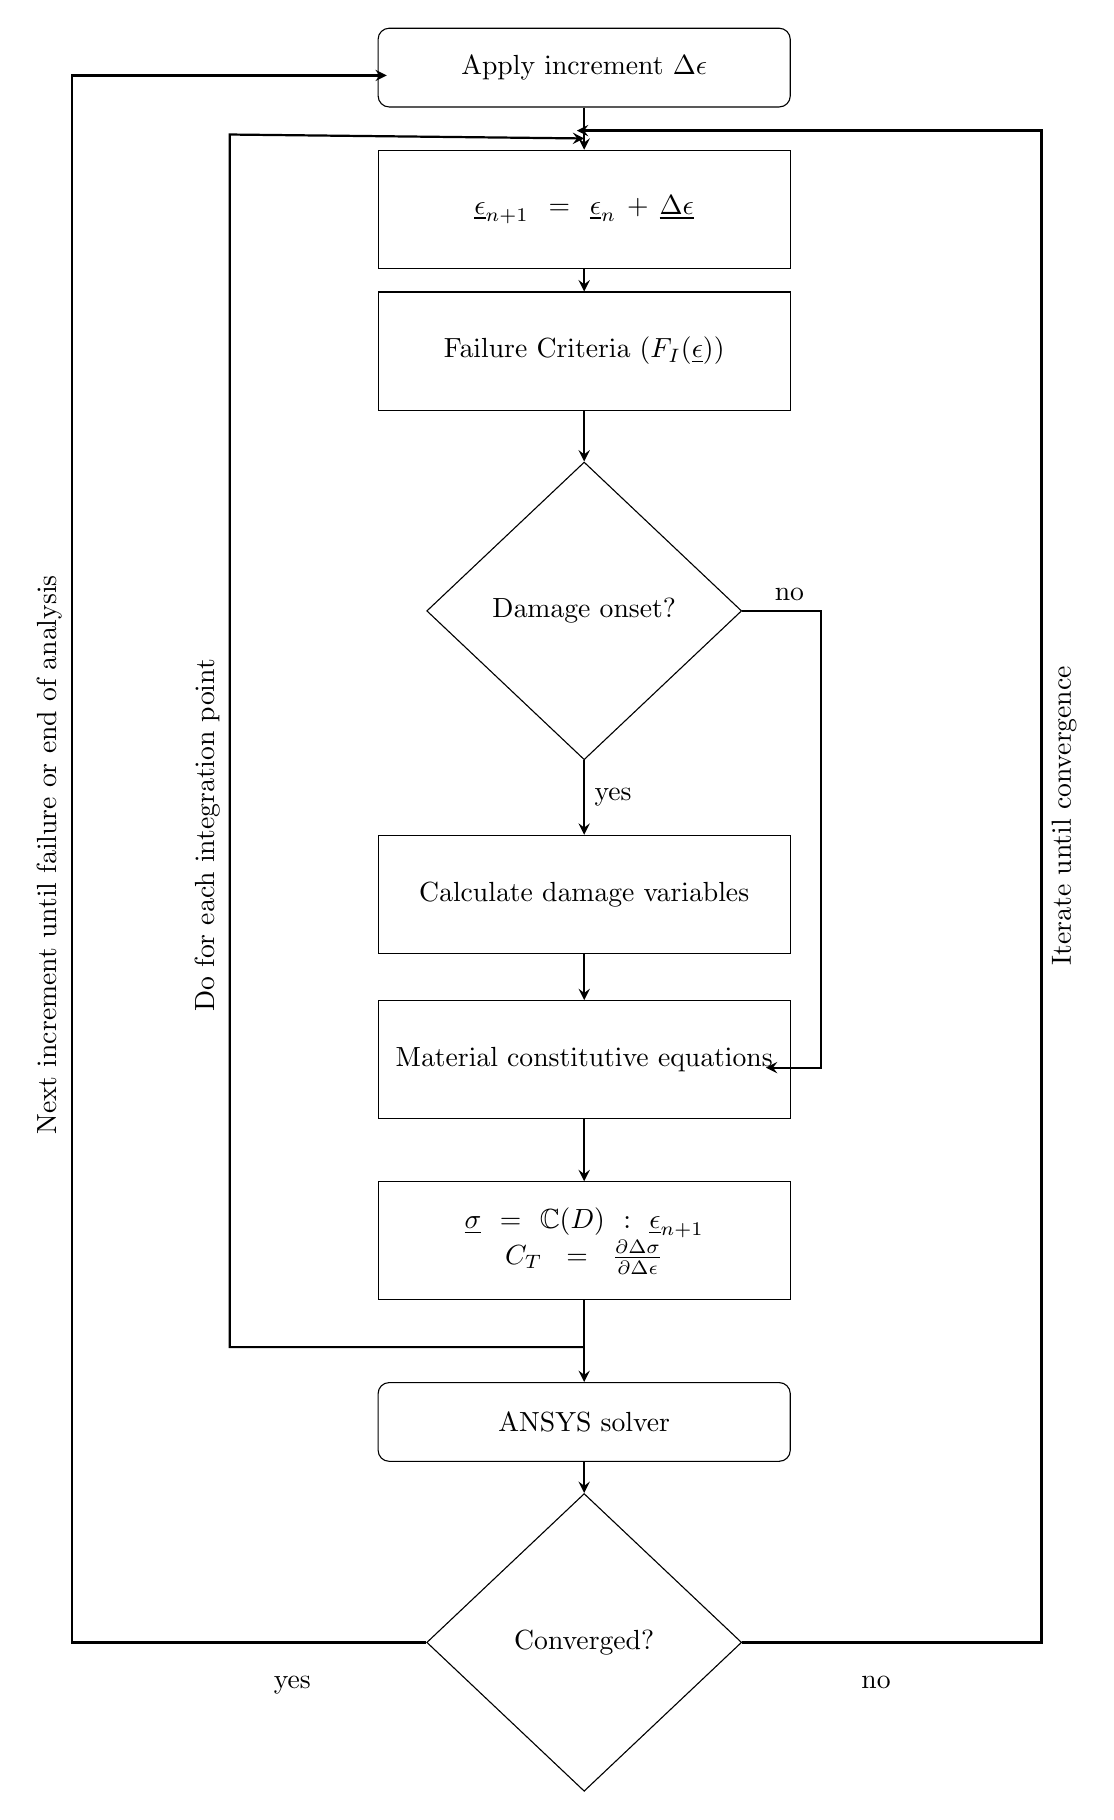
\begin{tikzpicture}[node distance = 1.8cm]

\node(straininc) [startstop] {Apply increment $\Delta\epsilon$};
\node(strainadd) [process, below of = straininc] {$\underline{\epsilon}_{n+1} = \underline{\epsilon}_{n} + \underline{\Delta\epsilon} $};
\node(Failure)   [process, below of = strainadd] {Failure Criteria ($F_{I}(\underline{\epsilon}))$};
\node(Damageon)  [decision, below of = Failure, yshift=-1.5cm] {Damage onset?};
\node(Damagecalc) [process, below of = Damageon, yshift=-1.8cm] {Calculate damage variables};
\node(Materialeqn)[process, below of = Damagecalc, yshift=-0.3cm] {Material constitutive equations};
\node(Tangent)[process, below of = Materialeqn, yshift=-0.5cm] { $\underline{\sigma} = \mathbb{C}(D):\underline{\epsilon}_{n + 1}$ \\ $C_{T}=\frac{\partial \Delta \sigma}{\partial \Delta \epsilon}$};
\node(abaqus)[startstop, below of = Tangent, yshift=-0.5cm] {ANSYS solver};
\node(Converge)[decision, below of = abaqus, yshift=-1cm] {Converged?};

\draw [arrow] (straininc) -- (strainadd);
\draw [arrow] (strainadd) -- (Failure);
\draw [arrow] (Failure) -- (Damageon);
\draw [arrow] (Damageon) -- node[anchor = west]{yes} (Damagecalc);
\draw [arrow] (Damagecalc) -- (Materialeqn);
\draw [arrow] (Materialeqn) -- (Tangent);
\draw [arrow] (Tangent) -- (abaqus);
\draw [arrow] (abaqus) -- (Converge);
\draw [arrow] (Damageon.east) node[xshift=0.6cm,anchor = south]{no} -| ++(1,-5.8) -- ++(-0.7,0)  (Materialeqn);

\draw [arrow] (Converge.west)node[xshift=-1.7cm,yshift=-0.3cm,anchor = north]{yes} -| node[xshift=10cm,sloped,above]{Next increment until failure or end of analysis}++(-4.5,19.9) -- ++ (4,0) (straininc); 

\draw [arrow] (Converge.east)node[xshift=1.7cm,yshift=-0.3cm,anchor = north]{no} -| node[xshift=10.5cm,sloped,below]{Iterate until convergence} ++(3.8,19.2)-- ++ (-5.9,0)  (straininc); 

\draw [arrow] (0,-16.25)-|node[xshift=6.5cm,sloped,above]{Do for each integration point}++(-4.5,15.4)--(-0,-0.9);

 
\end{tikzpicture}
\end{center}




\begin{center}
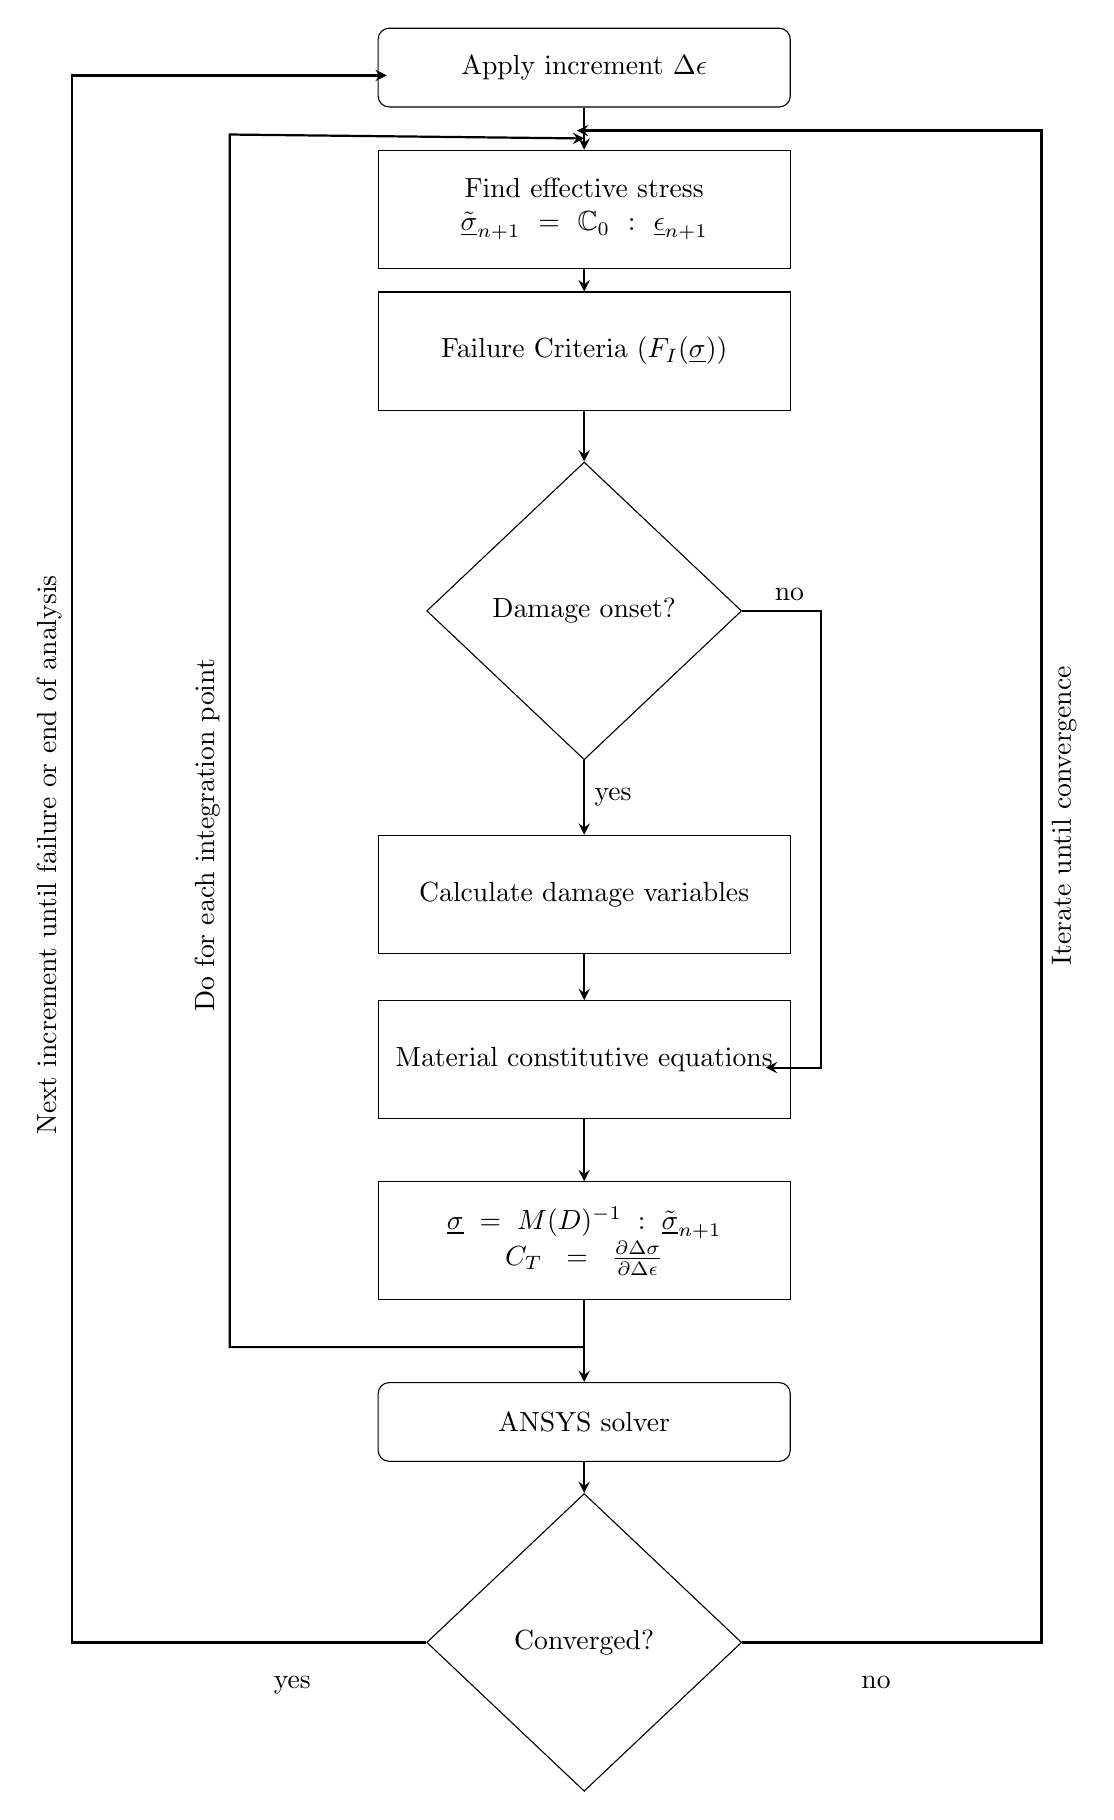
\begin{tikzpicture}[node distance = 1.8cm]

\node(straininc) [startstop] {Apply increment $\Delta\epsilon$};
\node(strainadd) [process, below of = straininc] {Find effective stress \\ $\underline{\tilde{\sigma}}_{n+1} = \mathbb{C}_{0} : \underline{\epsilon}_{n+1} $};
\node(Failure)   [process, below of = strainadd] {Failure Criteria ($F_{I}(\underline{\sigma}))$};
\node(Damageon)  [decision, below of = Failure, yshift=-1.5cm] {Damage onset?};
\node(Damagecalc) [process, below of = Damageon, yshift=-1.8cm] {Calculate damage variables};
\node(Materialeqn)[process, below of = Damagecalc, yshift=-0.3cm] {Material constitutive equations};
\node(Tangent)[process, below of = Materialeqn, yshift=-0.5cm] {$\underline{\sigma} = M(D)^{-1}:\underline{\tilde{\sigma}}_{n+1}$ \\  $C_{T}=\frac{\partial \Delta \sigma}{\partial \Delta \epsilon}$};
\node(abaqus)[startstop, below of = Tangent, yshift=-0.5cm] {ANSYS solver};
\node(Converge)[decision, below of = abaqus, yshift=-1cm] {Converged?};

\draw [arrow] (straininc) -- (strainadd);
\draw [arrow] (strainadd) -- (Failure);
\draw [arrow] (Failure) -- (Damageon);
\draw [arrow] (Damageon) -- node[anchor = west]{yes} (Damagecalc);
\draw [arrow] (Damagecalc) -- (Materialeqn);
\draw [arrow] (Materialeqn) -- (Tangent);
\draw [arrow] (Tangent) -- (abaqus);
\draw [arrow] (abaqus) -- (Converge);
\draw [arrow] (Damageon.east) node[xshift=0.6cm,anchor = south]{no} -| ++(1,-5.8) -- ++(-0.7,0)  (Materialeqn);

\draw [arrow] (Converge.west)node[xshift=-1.7cm,yshift=-0.3cm,anchor = north]{yes} -| node[xshift=10cm,sloped,above]{Next increment until failure or end of analysis}++(-4.5,19.9) -- ++ (4,0) (straininc); 

\draw [arrow] (Converge.east)node[xshift=1.7cm,yshift=-0.3cm,anchor = north]{no} -| node[xshift=10.5cm,sloped,below]{Iterate until convergence} ++(3.8,19.2)-- ++ (-5.9,0)  (straininc); 

\draw [arrow] (0,-16.25)-|node[xshift=6.5cm,sloped,above]{Do for each integration point}++(-4.5,15.4)--(-0,-0.9);

 
\end{tikzpicture}
\end{center}
\end{document}
